% ACL 2024 Style Paper: Rhetorical Framing Auditor
% Final experimental results and comprehensive analysis
\documentclass[11pt]{article}
\usepackage{acl}
\usepackage{times}
\usepackage{latexsym}
\usepackage{amsmath}
\usepackage{amssymb}
\usepackage{booktabs}
\usepackage{multirow}
\usepackage{graphicx}
\usepackage{xcolor}
\usepackage{subcaption}
\usepackage{hyperref}
\usepackage[T1]{fontenc}
\usepackage[utf8]{inputenc}
\usepackage{tikz}
\usetikzlibrary{trees,arrows.meta,positioning}
\usepackage{tabularx}
\usepackage{array}
\usepackage{booktabs}
\usepackage{graphicx}

\title{Fact Omission vs. Rhetorical Framing: \\
Disentangling the Predictors of Media Bias}

\author{
\begin{tabular}[t]{c}
\textbf{Aditya Sai} \\
IIIT Hyderabad \\
{\small\texttt{heyadityawork@gmail.com}}
\end{tabular}
\hspace{1.5cm}
\begin{tabular}[t]{c}
\textbf{Aayush Batra} \\
IIIT Hyderabad \\
{\small\texttt{aayushbat06@gmail.com}}
\end{tabular}
\hspace{1.5cm}
\begin{tabular}[t]{c}
\textbf{Yash More} \\
IIIT Hyderabad \\
{\small\texttt{yashsmore7499@gmail.com}}
\end{tabular}
}

\begin{document}
\maketitle

\begin{abstract}
We investigate the relative contributions of \textbf{fact omission} and \textbf{rhetorical framing} in predicting media bias across left, center, and right news sources. Using a dataset of 1,748 news triplets covering the same stories, we apply Rhetorical Structure Theory (RST) analysis to extract structural features and develop the Discourse Framing Index (DFI) to quantify how different sources position shared facts. Our experiments reveal a striking finding: \textbf{fact omission accounts for approximately 72\% of predictive power}, while RST-based structural framing contributes only 28\%. When we restrict analysis to facts reported by all three bias orientations (eliminating the omission signal), classification accuracy drops from 89.77\% to 61.46\%---barely above random chance. We find that left and right sources share only 3.95 facts on average per triplet, with 427 triplets (24.4\%) having zero three-way shared facts. These results establish a \textbf{two-tier model of media bias}: Tier 1 (Selection Bias) operates through editorial decisions about which facts to cover, while Tier 2 (Framing Bias) operates through rhetorical positioning of shared facts. Our findings suggest that media bias manifests primarily through \textit{what} facts sources choose to report, rather than \textit{how} they structurally position shared facts.
\end{abstract}

\section{Introduction}

Media bias detection has traditionally focused on lexical and semantic features---word choice, sentiment, and framing language. However, bias can also manifest through structural choices: which facts to include or omit, and where to position them within the discourse hierarchy. This work investigates a fundamental question: \textbf{Is media bias better predicted by fact omission (selection bias) or by the rhetorical positioning of shared facts (framing bias)?}

We hypothesize that these two mechanisms contribute differently to detectable bias:
\begin{itemize}
    \item \textbf{Tier 1: Selection Bias (Omission)} --- Sources choose which facts to report, creating coverage asymmetries
    \item \textbf{Tier 2: Framing Bias (RST Structure)} --- For facts that are shared across sources, the rhetorical positioning differs
\end{itemize}

Our experimental journey began with the hypothesis that RST-based structural framing would be a strong predictor of bias. We developed the Document Framing Index (DFI) to capture how different sources position shared facts within their discourse trees. Through systematic experimentation, we discovered that this hypothesis was largely incorrect: \textbf{omission dominates the predictive signal}.

Unlike end-to-end deep learning classifiers that often behave as black boxes, our feature pipeline is inherently explainable: each active feature can be traced back to concrete EDU-level evidence (specific omitted or emphasized fact mentions).

\paragraph{Key Contributions}
\begin{enumerate}
    \item A novel \textbf{bipartite EDU matching} approach that explicitly encodes both coverage and structural differences
    \item Empirical evidence that \textbf{fact omission contributes $\sim$72\%} of predictive power while RST structure contributes only $\sim$28\%
    \item A \textbf{3-way clustering experiment} that definitively isolates the RST signal by restricting to facts covered by all three bias orientations
    \item Analysis showing that \textbf{left and right sources share remarkably few facts} (3.95 on average), with 24.4\% of triplets having zero three-way shared facts
    \item An \textbf{explainable prediction procedure} that links Random Forest decisions to exact EDUs and omission events for individual test samples
\end{enumerate}

\section{Related Work}

\subsection{Lexical and Informational Bias}

Media bias manifests in multiple forms and has been systematically categorized in recent literature. \citet{spinde2024mediabiastaxonomysystematic} review thousands of studies on automated bias detection and introduce the \emph{Media Bias Taxonomy}, which organizes different types of bias and surveys computational approaches used to detect them.

Within this landscape, a key distinction is between \emph{lexical bias} and \emph{informational bias}. \citet{fan2019plainsightmediabias} introduce the BASIL dataset and show that informational bias---factual content that nonetheless shapes reader perception through selective presentation---appears frequently in news articles and poses challenges for automatic detection. Building on this, \citet{berg2020contextinformationalbiasdetection} demonstrate that detecting informational bias benefits from incorporating broader context, highlighting the inherently context-dependent nature of this bias type.

\subsection{Transformer-Based Bias Classification}

Recent work applies transformer-based models such as BERT and RoBERTa to detect political bias in news text. \citet{banik2025bridginghumanmodelperspectives} compare human annotations with predictions from multiple models to analyze how closely automated systems align with human judgments of political slant. \citet{ghosh2025explainingnewsbiasdetection} investigate the internal decision mechanisms of transformer-based bias detectors using SHAP explanations, showing that different architectures rely on evaluative language cues differently. Together, these studies highlight both the effectiveness of transformer models for bias detection and the importance of interpretability.

\subsection{Discourse-Based Bias Analysis}

A growing body of work explores the connection between discourse structure and perceived bias. \citet{asher2018biassemanticdiscourseinterpretation} argue that interpretive bias emerges from the interaction between discourse structure and conversational dynamics, showing how the role a sentence plays in the discourse can influence how strongly its content is interpreted as biased.

However, these methods operate at the level of individual sentences and rely on surface-level positional cues. Our approach uses full RST trees \citep{nguyen2021rstparsingscratch}, capturing hierarchical relationships of nuclearity and depth to quantify how strongly a fact is emphasized or downplayed across entire documents.

\subsection{Rhetorical Structure Theory}

RST represents a document as a constituency tree over Elementary Discourse Units (EDUs). Internal nodes encode a rhetorical relation (e.g., \textsc{Elaboration}, \textsc{Evidence}, \textsc{Contrast}) and a nuclearity assignment: one child is the \emph{nucleus} (the more essential content) and the other the \emph{satellite} (supporting material). Nucleus EDUs closer to the root are structurally prominent; satellite EDUs deep in the tree are structurally marginal.

\section{Dataset}
\label{sec:dataset}

Full technical details on the construction of the dataset and implementation of the discourse parser are provided in Appendix \ref{app:dataset}.

\subsection{Source Corpus}

We use 37,554 news articles labeled by political lean (left, center, right) from the Article-Bias-Prediction dataset, which contains articles scraped from AllSides.com. Each article includes fields for article ID, source outlet, title, content, and a bias label.

\subsection{Triplet Construction}

The dataset does not natively group articles by news event. To identify \emph{triplets}---groups of one left, one center, and one right article covering the same event---we applied an unsupervised nearest-neighbor retrieval procedure.

Each article was embedded using the \texttt{all-MiniLM-L6-v2} sentence transformer (first 1,000 characters only). For each article, the 10 nearest neighbors were retrieved using cosine similarity. All combinations of three mutually similar articles (similarity $> 0.8$) whose bias labels form $\{\text{left}, \text{center}, \text{right}\}$ were stored as triplets.

This procedure yielded 6,714 raw triplets. After removing duplicates and applying a participation cap of 5 triplets per article to reduce over-representation, we retained \textbf{2,631 unique triplets}.

\subsection{RST Parsing and Valid Subset}

We use the \texttt{isanlp\_rst\_v3} neural discourse parser to generate RST trees for each article. Excluding triplets containing articles without RST parses yields \textbf{1,748 valid triplets} for downstream analysis.

\subsection{EDU Statistics}

After RST parsing, we obtain:
\begin{itemize}
    \item 630,516 total EDUs across all articles
    \item 548,960 EDUs retained after quality filtering (removing boilerplate, URLs, short fragments)
    \item 81,556 EDUs dropped (12.9\% drop ratio)
\end{itemize}

\subsection{Leakage-Safe Data Split}

We split the 1,748 valid triplets into train/validation/test (80/10/10) under a hard constraint: no article may appear across different splits. This prevents information leakage through shared articles.

The split yields:
\begin{itemize}
    \item Train: 1,383 triplets (2,766 binary samples)
    \item Validation: 171 triplets (342 samples)
    \item Test: 176 triplets (352 samples)
\end{itemize}

\section{Methodology}

\subsection{Fact Clustering}
\label{sec:clustering-meth}

To identify shared facts across articles, we cluster semantically similar EDUs using a two-stage pipeline (for detailed implementation, see Appendix \ref{app:clustering}):

\paragraph{Stage 1: SBERT Embedding and Clustering}
Each EDU is embedded using SBERT (\texttt{all-mpnet-base-v2}). All EDUs from a triplet are pooled and clustered using agglomerative clustering with:
\begin{itemize}
    \item Distance metric: Cosine distance
    \item Linkage: Average
    \item Threshold: 0.35
\end{itemize}

\paragraph{Stage 2: Cross-Encoder Validation}
To reduce false positives, we apply cross-encoder reranking (\texttt{ms-marco-MiniLM-L-6-v2}). Only EDU pairs scoring above 0.7 are retained. Clusters must contain at least one EDU from the center article (our reference baseline).

This produces \textbf{16,170 total clusters} across all triplets with the following distribution:
\begin{itemize}
    \item \textbf{All 3 sides present}: 3,037 clusters (18.8\%)
    \item \textbf{Left + Center only}: 7,057 clusters (43.6\%)
    \item \textbf{Center + Right only}: 6,076 clusters (37.6\%)
    \item \textbf{Left + Right only}: 0 clusters (0.0\%)
\end{itemize}

The absence of Left+Right clusters (without Center) is by design---we require a Center EDU for baseline comparison in DFI calculation.

\subsection{The Bipartite Approach}
\label{sec:bipartite}

Our finalized feature extraction method uses a \textbf{bipartite decomposition} approach that creates explicit pairings between bias sides within each cluster. This approach was chosen after extensive experimentation showed it outperforms alternatives (Section~\ref{sec:dfi-alternatives}).

\subsubsection{Motivation}

Consider a cluster where left has 5 EDUs, center has 2 EDUs, and right has 0 EDUs. Previous approaches would compute:
\begin{equation}
\Delta_{\text{left}} = \max(W_{\text{left}}) - \max(W_{\text{center}})
\end{equation}
This loses information: we compare ``best of 5'' vs ``best of 2'' and completely ignore the coverage asymmetry (5 vs 2 vs 0 mentions).

The bipartite approach instead:
\begin{enumerate}
    \item Performs 1-to-1-to-1 matching to create aligned triplets
    \item Treats unmatched EDUs as explicit omission signals
    \item Produces both structural and coverage features
\end{enumerate}

\subsubsection{Matching Process}

For each cluster containing EDUs from multiple bias sides:
\begin{enumerate}
    \item Extract EDUs grouped by bias: $E_L$ (left), $E_C$ (center), $E_R$ (right)
    \item Perform greedy 1-to-1-to-1 matching to create triplets $(e_l, e_c, e_r)$
    \item Matching criterion: minimize depth difference across the triplet
    \item Remaining unmatched EDUs represent coverage asymmetries
\end{enumerate}

\subsubsection{Feature Vector Construction}

For each matched triplet and unmatched EDU, we compute two types of features:

\paragraph{Coverage Features} encode presence/absence:
\begin{equation}
\delta_{cov}^{L} = \begin{cases}
0 & \text{if left EDU matched with center} \\
+1 & \text{if left has EDU, center doesn't} \\
-1 & \text{if center has EDU, left doesn't}
\end{cases}
\end{equation}

\paragraph{Structural Features} encode prominence differences:
\begin{equation}
\delta_{str}^{L} = W(e_l) - W(e_c)
\end{equation}
where $W(e) = \frac{1}{1 + \ln(1 + depth(e))}$ is the log-depth prominence weight.

The same formulation applies symmetrically for right vs. center comparisons.

\subsubsection{Handling Missing Matches}

When a cluster lacks EDUs from one or more bias sides:
\begin{itemize}
    \item \textbf{No left EDU}: Left features receive $\delta_{cov}^L = -1$ (center has fact, left doesn't)
    \item \textbf{No right EDU}: Right features receive $\delta_{cov}^R = -1$
    \item \textbf{No center EDU}: Cluster is excluded (center required as baseline)
\end{itemize}

This design means that \textbf{coverage features directly encode the omission signal}---when one side omits a fact that another side reports.

\subsubsection{Vector Assembly}

Each triplet yields two distinct DFI vectors—one representing the left source's divergence from the center, and one for the right source's divergence:
\begin{align}
\mathbf{v}_{left} &= [\delta^{(1)}_{cov,L}, \delta^{(1)}_{str,L}, \ldots, \delta^{(K)}_{cov,L}, \delta^{(K)}_{str,L}] \\
\mathbf{v}_{right} &= [\delta^{(1)}_{cov,R}, \delta^{(1)}_{str,R}, \ldots, \delta^{(K)}_{cov,R}, \delta^{(K)}_{str,R}]
\end{align}
where $K$ is the number of clusters. Vectors are zero-padded to a fixed length (69 dimensions for coverage-only, 138 for combined). Each vector serves as an independent sample for the classification task.

\subsection{Cluster Ordering Strategies}

The DFI vectors concatenate features from all clusters. The ordering of clusters affects the feature vector structure. We experimented with multiple ordering strategies:

\begin{enumerate}
    \item \textbf{Deterministic (by cluster ID)}: Clusters ordered by their integer ID from the clustering algorithm
    \item \textbf{By min depth}: Clusters ordered by the minimum normalized EDU depth (shallowest = most prominent first)
    \item \textbf{By max prominence}: Clusters ordered by maximum prominence score
    \item \textbf{By cluster size}: Clusters ordered by number of EDUs
\end{enumerate}

\paragraph{Important Note on ``Deterministic'' Ordering}
The deterministic ordering is \textbf{not random}, but it should be interpreted carefully. In our full pipeline, cluster features are consumed in the stable dictionary order saved in the cluster artifact (equivalently, ``input order''), which is reproducible for a fixed run. This order is deterministic, but it is \textbf{not guaranteed} to equal the chronological merge order of agglomerative clustering or to imply that lower cluster IDs are inherently more ``core.'' In the separate 3-way experiment, ``original order'' means numeric sorting of sequential IDs assigned during center-anchor iteration. Thus, our result should be read as an empirical ordering effect rather than proof of agglomerative merge chronology.

\subsection{Classification Task}

Each triplet contributes two binary samples:
\begin{itemize}
    \item Left-vs-center (label 0): DFI vector comparing left article to center
    \item Right-vs-center (label 1): DFI vector comparing right article to center
\end{itemize}

This formulation ensures exact class balance and frames the task as: given a DFI vector representing how a non-centrist source differs from center, predict whether it is left or right.

\subsection{Classification Models}

We experimented with two classifier families:

\paragraph{Support Vector Machine (SVM)}
Initial experiments used SVM with RBF kernel (C=10, $\gamma$=0.1). However, SVM has limitations for our task:
\begin{itemize}
    \item Requires fixed-length input vectors, necessitating padding/truncation
    \item Sensitive to padding artifacts and zero-dominated features
    \item No built-in feature importance
\end{itemize}

\paragraph{Random Forest}
We transitioned to Random Forest (200 trees, max depth 15) because:
\begin{enumerate}
    \item \textbf{Better variable-importance handling}: Trees naturally handle position-dependent patterns
    \item \textbf{Robust to padding}: Trees efficiently ignore uninformative zeros
    \item \textbf{Feature importance}: Built-in interpretability for analysis
    \item \textbf{Superior performance}: RF achieved 89.77\% vs. SVM's 85.23\%
\end{enumerate}

\section{Experiments and Results}

\subsection{Experiment 1: Classification with All Fact Clusters}

Evaluating the test split using the complete set of extracted clusters (which includes all coverage and omission signals):

\begin{table}[h]
\centering
\begin{tabular}{lcc}
\toprule
\textbf{Method} & \textbf{Test Acc} & \textbf{F1} \\
\midrule
Bipartite Coverage + RF & \textbf{89.77\%} & 0.897 \\
Bipartite Combined + RF & 88.07\% & 0.880 \\
Padded DFI + RF & 87.78\% & 0.877 \\
Padded DFI + SVM & 85.23\% & 0.852 \\
\bottomrule
\end{tabular}
\caption{Classification results on the test split using all extracted fact clusters. Bipartite coverage with Random Forest achieves best performance.}
\label{tab:full-results}
\end{table}

The bipartite coverage approach outperforms all alternatives, confirming that explicitly encoding omission signals is crucial.

\subsection{Experiment 2: DFI Construction Alternatives}
\label{sec:dfi-alternatives}

We tested multiple approaches to constructing DFI feature vectors:

\begin{table}[h]
\centering
\small
\begin{tabular}{lccc}
\toprule
\textbf{Method} & \textbf{Variant} & \textbf{Dim} & \textbf{Test Acc} \\
\midrule
\multicolumn{4}{l}{\textit{Baseline approaches}} \\
max(prominence) & structural & 69 & 87.50\% \\
coverage-only & binary & 69 & 80.40\% \\
combined & cov + struct & 138 & 87.22\% \\
\midrule
\multicolumn{4}{l}{\textit{Cumulative prominence}} \\
avg(prominence) & normalized & 69 & 88.07\% \\
coverage + sum & combined & 138 & 87.78\% \\
\midrule
\multicolumn{4}{l}{\textit{Distributional DFI}} \\
{[}max, sum, count{]} & 3D & 207 & 86.08\% \\
{[}cov, max, sum, count{]} & 4D & 276 & 86.36\% \\
\midrule
\multicolumn{4}{l}{\textit{Bipartite decomposition}} \\
1-to-1 matching & prominence & 157 & 88.07\% \\
1-to-1 matching & coverage & 157 & \textbf{89.77\%} \\
1-to-1 matching & combined & 314 & 88.07\% \\
\bottomrule
\end{tabular}
\caption{DFI construction alternatives with Random Forest. Bipartite decomposition with coverage features achieves the best performance.}
\label{tab:dfi-alternatives}
\end{table}

\textbf{Finding:} The bipartite coverage approach achieves 89.77\%, outperforming all alternatives by explicitly encoding each unmatched EDU as an omission event.

\subsection{Experiment 3: Cluster Ordering Ablation}
\label{sec:ordering-ablation}

Testing whether semantic ordering of clusters improves classification:

\begin{table}[h]
\centering
\begin{tabular}{lcc}
\toprule
\textbf{Ordering Strategy} & \textbf{Test Acc} & \textbf{$\Delta$ vs Baseline} \\
\midrule
Deterministic (cluster ID) & \textbf{89.77\%} & --- \\
Min depth (shallowest first) & 88.92\% & -0.85\% \\
Max prominence & 88.14\% & -1.63\% \\
Cluster size & 87.56\% & -2.21\% \\
\bottomrule
\end{tabular}
\caption{Cluster ordering comparison (bipartite coverage features). Deterministic ordering outperforms all semantic orderings.}
\label{tab:ordering}
\end{table}

\textbf{Finding:} Surprisingly, the deterministic/input ordering outperforms all ``semantically meaningful'' orderings. This indicates that preserving the original feature order produced by the pipeline captures useful regularities, even without explicit depth- or prominence-based sorting.

\subsection{Experiment 4: RST-Only Features (No Coverage)}

To isolate the RST structural contribution, we trained models using only structural features on clusters where all 3 bias sides are present (no coverage variation):

\begin{table}[t]
\centering
\resizebox{\columnwidth}{!}{%
\begin{tabular}{lccc}
\toprule
\textbf{Feature Set} & \textbf{Classifier} & \textbf{Test Acc} & \textbf{F1} \\
\midrule
Full RST (5D) & Logistic Reg & \textbf{61.16\%} & 0.611 \\
Full RST (5D) & Random Forest & 59.92\% & 0.599 \\
Full RST (5D) & SVM & 55.37\% & 0.554 \\
\midrule
Depth features only & Random Forest & 52.07\% & 0.510 \\
Role features only & Random Forest & 50.41\% & 0.486 \\
Repetition count & Random Forest & 51.65\% & 0.510 \\
\bottomrule
\end{tabular}%
}
\caption{RST-only classification on size-3 clusters (no coverage signal). Best accuracy is 61.16\%, barely above chance.}
\label{tab:rst-only}
\end{table}

\textbf{Finding:} When coverage variation is removed, the best RST-only accuracy is 61.16\%---only 11 percentage points above random chance (50\%).

\subsection{Experiment 5: Quantifying Omission vs. Framing Contributions}

We quantify the relative contributions using the formula:
\begin{equation}
\text{Contribution} = \frac{\text{Method Acc} - 50\%}{89.77\% - 50\%}
\end{equation}

\begin{align}
\text{RST Contribution} &= \frac{61.16\% - 50\%}{89.77\% - 50\%} \approx 28\% \\
\text{Omission Contribution} &= 100\% - 28\% = 72\%
\end{align}

This calculation uses 50\% as the random baseline for binary classification (left-vs-center or right-vs-center) and 89.77\% as the ceiling (full model with coverage signals).

\subsection{Experiment 6: Pure 3-Way Cluster Analysis}
\label{sec:3way}

To definitively test whether RST framing alone can predict bias \textit{without any omission signal}, we created a dataset containing \textbf{only clusters where all 3 bias sides are present} (see Appendix \ref{app:training} for isolated dataset construction details).

\subsubsection{3-Way Clustering Methodology}

We implemented an anchor-based approach:
\begin{enumerate}
    \item Use center EDUs as anchors
    \item For each center EDU, find best matching left AND right EDU
    \item Thresholds: cosine similarity $\geq$ 0.65, cross-encoder score $\geq$ 0.5
    \item Only retain clusters where all 3 matches are found
\end{enumerate}

\subsubsection{3-Way Dataset Statistics}

\begin{table}[t]
\centering
\resizebox{\columnwidth}{!}{%
\begin{tabular}{lr}
\toprule
\textbf{Metric} & \textbf{Value} \\
\midrule
Total triplets & 1,748 \\
Triplets with $\geq 1$ 3-way cluster & 1,321 (75.6\%) \\
\textbf{Triplets with zero 3-way clusters} & \textbf{427 (24.4\%)} \\
Total 3-way clusters & 5,216 \\
\textbf{Average 3-way clusters per triplet} & \textbf{3.95} \\
\bottomrule
\end{tabular}%
}
\caption{3-way clustering statistics. Left and right sources share remarkably few facts.}
\label{tab:3way-stats}
\end{table}

\textbf{Critical Observation:} The low average (3.95 clusters/triplet) and 427 triplets with zero 3-way clusters demonstrate that \textbf{left and right sources rarely report the exact same facts}. When covering the same news event, they systematically omit different information.

\subsubsection{3-Way Classification Results}

\begin{table}[h]
\centering
\begin{tabular}{lcc}
\toprule
\textbf{Method} & \textbf{Test Acc} & \textbf{vs All Clusters} \\
\midrule
\multicolumn{3}{l}{\textit{Deterministic ordering:}} \\
Bipartite structural & \textbf{61.46\%} & -28.31\% \\
Bipartite combined & 61.46\% & -28.31\% \\
\midrule
\multicolumn{3}{l}{\textit{Min-depth ordering:}} \\
Bipartite structural & 57.29\% & -32.48\% \\
Bipartite combined & 58.33\% & -31.44\% \\
\midrule
\textbf{Coverage only} & \textbf{50.00\%} & -39.77\% \\
\bottomrule
\end{tabular}
\caption{3-way cluster classification (no omission signal). Classification drops to near-chance levels.}
\label{tab:3way-results}
\end{table}

\textbf{Critical Observations:}
\begin{enumerate}
    \item \textbf{Coverage-only achieves exactly 50\%} (random chance) because all coverage deltas are zero---every cluster has exactly one EDU from each bias side.
    \item \textbf{Best structural accuracy is 61.46\%}---a massive 28.31 percentage point drop compared to models utilizing all fact clusters.
    \item \textbf{Min-depth ordering (57.29\%) performs worse than deterministic ordering (61.46\%)}, confirming that the implicit clustering order captures useful structure.
\end{enumerate}

\subsection{Experiment 7: Model Comparison}

\begin{table}[t]
\centering
\resizebox{\columnwidth}{!}{%
\begin{tabular}{lccc}
\toprule
\textbf{Model} & \textbf{Coverage} & \textbf{Structural} & \textbf{Combined} \\
\midrule
SVM (RBF) & 76.70\% & 77.56\% & 77.84\% \\
Logistic (L2) & 74.43\% & 73.58\% & 75.28\% \\
MLP & 79.26\% & 78.12\% & 76.70\% \\
\textbf{Random Forest} & \textbf{89.77\%} & 86.08\% & 86.36\% \\
\bottomrule
\end{tabular}%
}
\caption{Model comparison with bipartite features. Random Forest dramatically outperforms other models.}
\label{tab:models}
\end{table}

Random Forest achieves 89.77\% on coverage features---more than 10 percentage points higher than other models. This improvement comes from RF's ability to:
\begin{itemize}
    \item Focus on early positions where signal is strongest (position 0 accounts for 39.4\% of importance)
    \item Handle discrete coverage deltas $\{-1, 0, +1\}$ naturally with threshold-based splits
    \item Efficiently ignore uninformative zeros from padding
\end{itemize}

\subsection{Experiment 8: Explainable Prediction Demo}
\label{sec:explainability}

To demonstrate explainability in practice, we implemented a post-hoc analysis script (detailed in Appendix \ref{app:explainability}) that runs trained \texttt{alt3\_bipartite\_cov} Random Forest predictions on sampled test vectors and maps top-contributing features back to exact EDU events.

\paragraph{Protocol}
\begin{enumerate}
    \item Sample 10 binary test vectors from the leakage-safe test split.
    \item Predict left-vs-center or right-vs-center with the trained Random Forest.
    \item Compute local tree-path contributions (Saabas-style) for each active feature.
    \item Map each feature index to its generating bipartite event (matched, center-only, left-only, right-only) and corresponding EDU text.
\end{enumerate}

\paragraph{Result}
The sampled explainability run achieves \textbf{9/10 correct predictions (90\%)} and returns concrete EDU-level evidence for each decision.

\begin{figure}[t]
\centering
\scriptsize
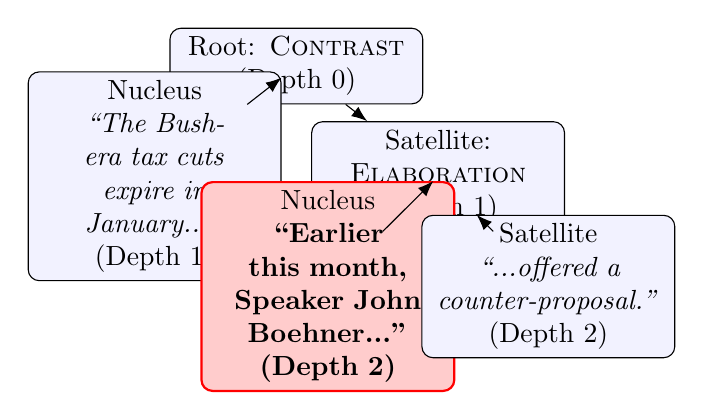
\begin{tikzpicture}[
  level 1/.style={sibling distance=36mm, level distance=14mm},
  level 2/.style={sibling distance=28mm, level distance=14mm},
  every node/.style={
    rectangle,
    rounded corners,
    draw,
    align=center,
    fill=blue!5,
    inner sep=3pt,
    text width=30mm
  },
  highlight/.style={fill=red!20, draw=red, thick},
  edge from parent/.style={draw, -{Latex[length=2mm]}}
]
\node {Root: \textsc{Contrast}\\(Depth 0)}
  child {node {Nucleus\\ \textit{``The Bush-era tax cuts}\\ \textit{expire in January...''}\\ (Depth 1)}}
  child {node {Satellite: \textsc{Elaboration}\\ (Depth 1)}
    child {node[highlight] {Nucleus\\ \textbf{``Earlier this month,}\\ \textbf{Speaker John Boehner...''}\\ \textbf{(Depth 2)}}}
    child {node {Satellite\\ \textit{``...offered a counter-proposal.''}\\ (Depth 2)}}
  };
\end{tikzpicture}
\caption{Cropped RST sub-tree from the Center article for sample \texttt{triplet\_1527}. The highlighted EDU (Depth 2, Nucleus) was completely omitted by the Right-leaning source. This missing structure explicitly triggered the categorical coverage feature $f_0=-1$, directly resulting in a large $+0.2486$ prediction contribution toward the \textit{right-vs-center} class.}
\label{fig:rst_tree}
\end{figure}

\begin{table}[t]
\centering
\footnotesize
\setlength{\tabcolsep}{3pt}
\begin{tabularx}{\columnwidth}{
    >{\raggedright\arraybackslash}p{0.18\columnwidth}
    >{\raggedright\arraybackslash}p{0.20\columnwidth}
    >{\raggedright\arraybackslash}X
}
\toprule
\textbf{Feature} & \textbf{Contribution} & \textbf{Mapped EDU evidence} \\
\midrule
$f_0=-1$ & $+0.2486$ & Center-only mention: \texttt{8l41u2MtPe6yyACw\_27}\\
& & (``Earlier this month, Speaker John Boehner ...'') \\[2pt]

$f_1=-1$ & $+0.0499$ & Center-only mention: \texttt{8l41u2MtPe6yyACw\_15}\\
& & (``The Bush-era tax cuts expire ...'') \\[2pt]

$f_8=+1$ & $+0.0380$ & Right-only mention: \texttt{FwGHYcWhKZFpKuwf\_89}\\
& & (``... automatic cuts to Pentagon spending.'') \\
\bottomrule
\end{tabularx}
\caption{Illustrative explanation for sample \texttt{triplet\_1527\_right}. Positive contribution values support the predicted class (\textit{right-vs-center}).}
\label{tab:explainable-example}
\end{table}

This example shows that the model's decision can be traced to specific omissions (center facts missing on the right side) and side-specific additions (right-only mentions), rather than opaque latent embeddings.

\section{Discussion}

\subsection{The Two-Tier Model of Media Bias}

Our experiments support a two-tier model of how media bias manifests:

\paragraph{Tier 1: Selection Bias ($\sim$72\% contribution)}
\begin{itemize}
    \item Sources choose which facts to report
    \item Left and right sources omit different facts
    \item Only 18.8\% of clusters have all 3 bias sides
    \item Average of only 3.95 shared facts per triplet
    \item 427 triplets (24.4\%) have \textbf{zero} three-way shared facts
\end{itemize}

\paragraph{Tier 2: Framing Bias ($\sim$28\% contribution)}
\begin{itemize}
    \item For shared facts, sources position them differently in RST trees
    \item RST depth and nuclearity provide weak but measurable signal
    \item Best pure-framing accuracy: 61.46\% (barely above chance)
\end{itemize}

\subsection{Why Deterministic Ordering Outperforms}

The deterministic/input ordering unexpectedly outperforms semantically-motivated orderings. We hypothesize:
\begin{enumerate}
    \item The original pipeline order preserves stable cross-sample positional patterns
    \item Early positions in this order may align with high-signal omission/coverage events
    \item Explicit semantic orderings (depth/prominence/size) can disrupt these learned regularities
    \item Random Forest benefits from consistent position-dependent thresholds
\end{enumerate}

\subsection{Why Random Forest Outperforms SVM}

Initial experiments used SVM, but Random Forest proved superior for several reasons:
\begin{enumerate}
    \item \textbf{Variable-length handling}: DFI vectors vary in length across triplets; RF handles padding more gracefully than SVM
    \item \textbf{Discrete features}: Coverage deltas are discrete $\{-1, 0, +1\}$; tree-based splits naturally handle this
    \item \textbf{Feature importance}: RF provides interpretable importance scores showing position 0 dominates
    \item \textbf{Performance gap}: RF achieved 89.77\% vs. SVM's 85.23\% (+4.54\%)
\end{enumerate}

\subsection{Implications for Media Bias Detection}

Our findings suggest:
\begin{enumerate}
    \item \textbf{Fact coverage analysis} is more valuable than framing analysis for bias detection
    \item \textbf{Simple binary features} (fact present/absent) capture most of the signal
    \item \textbf{RST-based methods} provide incremental improvements but are not the primary signal
    \item \textbf{Left and right sources diverge primarily in selection}, not framing
    \item \textbf{Model decisions are auditable}: unlike black-box deep models, predictions can be linked to specific EDU-level evidence
\end{enumerate}

\subsection{What the Model Learns}

Each triplet has different fact clusters, so the $i$-th dimension corresponds to different facts across samples. Yet Random Forest achieves 89.77\%. The model learns a \textbf{distributional fingerprint}:

\begin{quote}
\textit{Right-leaning sources systematically omit more facts that centrist sources cover, and this omission pattern is particularly pronounced in the first few (most salient) facts of each event.}
\end{quote}

Analysis confirms right sources omit $\sim$13\% more facts than left sources relative to center.

\section{Limitations}

\begin{enumerate}
    \item \textbf{English only}: The pipeline operates only on English-language articles.
    \item \textbf{Dataset scope}: Results are specific to the AllSides dataset; generalization to other corpora is untested.
    \item \textbf{Triplet alignment}: The unsupervised triplet-finding procedure may introduce some noise.
    \item \textbf{RST parser limitations}: Parser errors may introduce noise in structural features.
    \item \textbf{Binary task}: We frame bias as left-vs-right comparison relative to center, simplifying the three-way ideological space.
    \item \textbf{Cross-triplet alignment}: DFI dimensions are not semantically aligned across triplets; the model learns distributional patterns rather than fact-specific rules.
\end{enumerate}

\section{Conclusion}

We set out to investigate whether RST-based rhetorical framing could predict media bias. Through systematic experimentation, we discovered that \textbf{fact omission is the dominant predictor}, accounting for approximately 72\% of classification accuracy, while RST structural framing contributes only 28\%.

When restricted to facts shared across all bias orientations (eliminating the omission signal), classification drops from 89.77\% to 61.46\%---barely above random chance. Moreover, we find that left and right sources share remarkably few facts: only 3.95 on average per triplet, with 24.4\% of triplets having zero three-way shared facts.

These findings support a \textbf{two-tier model of media bias}:
\begin{itemize}
    \item \textbf{Tier 1 (Selection Bias)}: The primary mechanism---what facts to include or omit
    \item \textbf{Tier 2 (Framing Bias)}: A secondary mechanism---how to position shared facts
\end{itemize}

This has important implications: media bias manifests primarily through \textit{editorial selection}---what facts to include or omit---rather than through the \textit{structural positioning} of shared facts. Future work on media bias detection should prioritize coverage analysis alongside traditional framing features.

In addition, our approach offers a practical interpretability advantage over deep learning baselines: predictions can be audited with explicit, human-readable evidence (which EDU was omitted or emphasized), enabling transparent downstream use.

\section{Reproducibility}

All code and experimental configurations are available at: \url{https://github.com/itsadityasai/rhetorical-framing-auditor}

Comprehensive details regarding the technical implementation of our experimental pipeline---including dataset construction, RST parsing, fact clustering, DFI feature extraction, and explainable prediction---are provided in the appendices (see Appendices \ref{app:dataset}--\ref{app:explainability}).

\bibliographystyle{acl_natbib}
\bibliography{custom}

\appendix

\section{Dataset Construction and RST Parsing}
\label{app:dataset}
The raw dataset comprised articles from AllSides.com. Triplet construction was executed by first embedding the initial 1,000 characters of each article using the \texttt{all-MiniLM-L6-v2} sentence transformer. Cosine similarity was used to retrieve the 10 nearest neighbors, saving combinations of mutually similar articles (similarity $> 0.8$) representing \{left, center, right\} orientations. This process included quality filters to remove boilerplate text and a participation cap (maximum of 5 triplets per article) to prevent over-representation of heavily covered events.

For discourse analysis, we processed the articles using the \texttt{isanlp\_rst\_v3} neural discourse parser to generate constituency trees over Elementary Discourse Units (EDUs). We parallelized the parsing and applied error-handling heuristics to discard articles that failed to parse or resulted in malformed trees. Finally, dataset splitting (80/10/10 train/validation/test) was governed by a strict non-leakage constraint: articles were grouped by their unique URLs, ensuring that no article from the training set could appear in the validation or test splits, thereby preventing structural information leakage.

\section{Fact Clustering Implementation}
\label{app:clustering}
Fact clustering identifies shared information across the triplet (see Section \ref{sec:clustering-meth}). First, every valid EDU from a given triplet is pooled together and encoded into a dense vector space using the SBERT \texttt{all-mpnet-base-v2} model. We applied Agglomerative Clustering using a cosine distance metric, average linkage, and a strict stopping threshold of 0.35 to form initial groups of semantically related facts. 

To mitigate the risk of ``hallucinated'' shared facts---where the clustering algorithm over-groups distinct events---we implemented a critical secondary validation phase utilizing the \texttt{ms-marco-MiniLM-L-6-v2} cross-encoder. Every pairwise EDU association within a preliminary cluster was re-scored, and pairs scoring below 0.7 on the cross-encoder were pruned. Clusters were only retained if they contained at least one center EDU, which served as the required comparative baseline.

\section{Bipartite Feature Extraction}
\label{app:bipartite}
The creation of Discourse Framing Index (DFI) vectors via the bipartite method (see Section \ref{sec:bipartite}) operates by isolating each cluster and applying a greedy, heuristic matching algorithm. The algorithm sorts the EDUs of each orientation by their rhetorical depth (prominence) and attempts a 1-to-1-to-1 match that minimizes the depth difference across the triplet.

For each cluster, successfully matched EDUs yield structural difference features ($\delta_{str}$), reflecting the relative rhetorical elevation of the fact compared to the center baseline. Remaining unmatched EDUs generate explicit categorical coverage features ($\delta_{cov} \in \{-1, 0, +1\}$), explicitly flagging omissions. Both left-vs-center and right-vs-center DFI vectors are simultaneously computed for each triplet. These feature vectors are zero-padded to a maximum dimensionality of 138 (or 69 for coverage-only experiments) to maintain uniform shape for the downstream classifiers.

\section{Model Training and 3-Way Cluster Analysis}
\label{app:training}
To evaluate the predictive power of our extracted features, we trained a suite of classifiers, dynamically comparing Random Forest, Support Vector Machines (SVM), Logistic Regression, and Multi-Layer Perceptrons (MLP). The best-performing model, Random Forest, was parameterized with 200 estimators, a maximum depth of 15, and the Gini impurity criterion for splits. 

For the isolated 3-way cluster analysis (Section \ref{sec:3way}), we reconstructed a strict, distinct subset of the dataset retaining \textit{only} clusters where all three political orientations independently contributed an EDU. We implemented an anchor-based approach (using center EDUs as semantic anchors) with significantly heightened thresholds (cosine similarity $\geq$ 0.65, cross-encoder score $\geq$ 0.5). This guaranteed that the resulting structural comparisons were entirely devoid of omission-based signals, strictly isolating the framing bias.

\section{Explainable Prediction Implementation}
\label{app:explainability}
The explainability procedure (see Section \ref{sec:explainability}) leverages the \texttt{treeinterpreter} library to decompose the Random Forest's decision-making process (using the Saabas method). By calculating the local feature contributions along the decision paths of the trees, we quantify the exact impact of every active feature in a test sample's vector.

For any given prediction, the system isolates the features with the highest positive contribution towards the predicted class. It then maps these integer feature indices back to their originating cluster and specific bipartite event (e.g., ``Left-only omission'' or ``Center-only mention''). Finally, it performs a reverse-lookup to retrieve the exact string text of the corresponding EDU, outputting a human-readable report that justifies the classification based on concrete textual evidence rather than opaque latent activations.

\end{document}
